\section{Overview}
This report contains figures related to the calibration
process of autocorrelator data from Odin-SMR.\\
\newline
The topic examined is:\\
\newline
Calibration of sky signals using linear and quadratic interpolations\\
The calibration of sky signals using two different interpolation
methods are compared.
The results from the two methods are very comparable
(depending a bit on the settings for the quadratic interpolation),
with statistically similar mean and median values
and similar distribution.


\clearpage
\newpage

\section{Calibration of sky signals}
We know from earlier studies that mean values
of calibrated sky signals differs somewhat from 
the expected \(T_{sky}\sim0 K\). In this report we examine
if a weighted quadratic interpolation routine
will improve the results.   



\subsection{Basics}
The calibration of sky signals is done by:
\begin{equation}
\label{eq:skysig}
T^{'}_{sky}=\frac{c_{sky}-c^{'}_{sky}}{g^{'}}+T_{sky}\approx(\frac{g}{g^{'}}-1)T_{sys},
\end{equation}
where \(T^{'}_{sky}\) is the estimation of the brightness temperature
of the sky signal, \(c_{sky}\approx g(T_{sys}+T_{sky})\approx gT_{sys}\) is the measured sky signal,
 \(c^{'}_{sky}\) is the reference estimated sky signal
which is retrieved using linear/quadratic interpolation using
the measured sky signals around the target \(c_{sky}\),   
\(g\) is the true
gain, and \(g^{'}\) is the estimated gain, \(T_{sys}\) is the system
noise temperature.
\subsection{Reference interpolation}
For each channel (\(c_{i}\)) of the autocorrelators 
we fit a second degree polynomial,
\begin{equation}
c_{i}(t)=a+bt+ct^{2},
\end{equation}
to the time series of reference measurements (\(c_{i}(t_{0})\),\(c_{i}(t_{1})\),...,\(c_{i}(t_{n})\)). For time zero a weighted quadratic fit can 
be estimated as
\begin{equation}
c_{i}(0)=\frac{1}{\Delta}\left|
\begin{array}{ccc}
\sum \frac{c_{i}(t_{j})w^{2}(t_{j})}{\sigma^{2}(t_{j})} & 
\sum \frac{t_{j}c_{i}(t_{j})w^{2}(t_{j})}{\sigma^{2}(t_{j})} &
\sum \frac{t_{j}^{2}c_{i}(t_{j})w^{2}(t_{j})}{\sigma^{2}(t_{j})}\\
\sum \frac{t_{j}c_{i}(t_{j})w^{2}(t_{j})}{\sigma^{2}(t_{j})} & 
\sum \frac{t_{j}^{2}c_{i}(t_{j})w^{2}(t_{j})}{\sigma^{2}(t_{j})} &
\sum \frac{t_{j}^{3}c_{i}(t_{j})w^{2}(t_{j})}{\sigma^{2}(t_{j})}\\
\sum \frac{t_{j}^{2}c_{i}(t_{j})w^{2}(t_{j})}{\sigma^{2}(t_{j})} & 
\sum \frac{t_{j}^{3}c_{i}(t_{j})w^{2}(t_{j})}{\sigma^{2}(t_{j})} &
\sum \frac{t_{j}^{4}c_{i}(t_{j})w^{2}(t_{j})}{\sigma^{2}(t_{j})}\\
\end{array}
\right|,
\end{equation}

\begin{equation}
\Delta=\left|
\begin{array}{ccc}
\sum \frac{w^{2}(t_{j})}{\sigma^{2}(t_{j})} & 
\sum \frac{t_{j}w^{2}(t_{j})}{\sigma^{2}(t_{j})} &
\sum \frac{t_{j}^{2}w^{2}(t_{j})}{\sigma^{2}(t_{j})}\\
\sum \frac{t_{j}w^{2}(t_{j})}{\sigma^{2}(t_{j})} & 
\sum \frac{t_{j}^{2}w^{2}(t_{j})}{\sigma^{2}(t_{j})} &
\sum \frac{t_{j}^{3}w^{2}(t_{j})}{\sigma^{2}(t_{j})}\\
\sum \frac{t_{j}^{2}w^{2}(t_{j})}{\sigma^{2}(t_{j})} & 
\sum \frac{t_{j}^{3}w^{2}(t_{j})}{\sigma^{2}(t_{j})} &
\sum \frac{t_{j}^{4}w^{2}(t_{j})}{\sigma^{2}(t_{j})}\\
\end{array}
\right|,
\end{equation}
and we use an exponential drop off weighting
\begin{equation}
w(t_{j})=exp\left(-\frac{|t_{j}|}{\lambda} \right),
\end{equation}
where \(\lambda\) controls the weighting,
and \(\sigma(t_{j})\) represents the uncertainty of each measurement
\begin{equation}
\sigma(t_{j})\sim\frac{1}{\sqrt{t_{int}}},
\end{equation}
where \(t_{int}\) is the integration time.

\subsection{Test results}

In this section we compare calibration of sky signals
using linear interpolation and the previously described
quadratic interpolation. Data from six orbits, including around
10000 sky signals, are considered. 


\subsubsection{Linear interpolation}
\begin{figure}[!t]
\centering
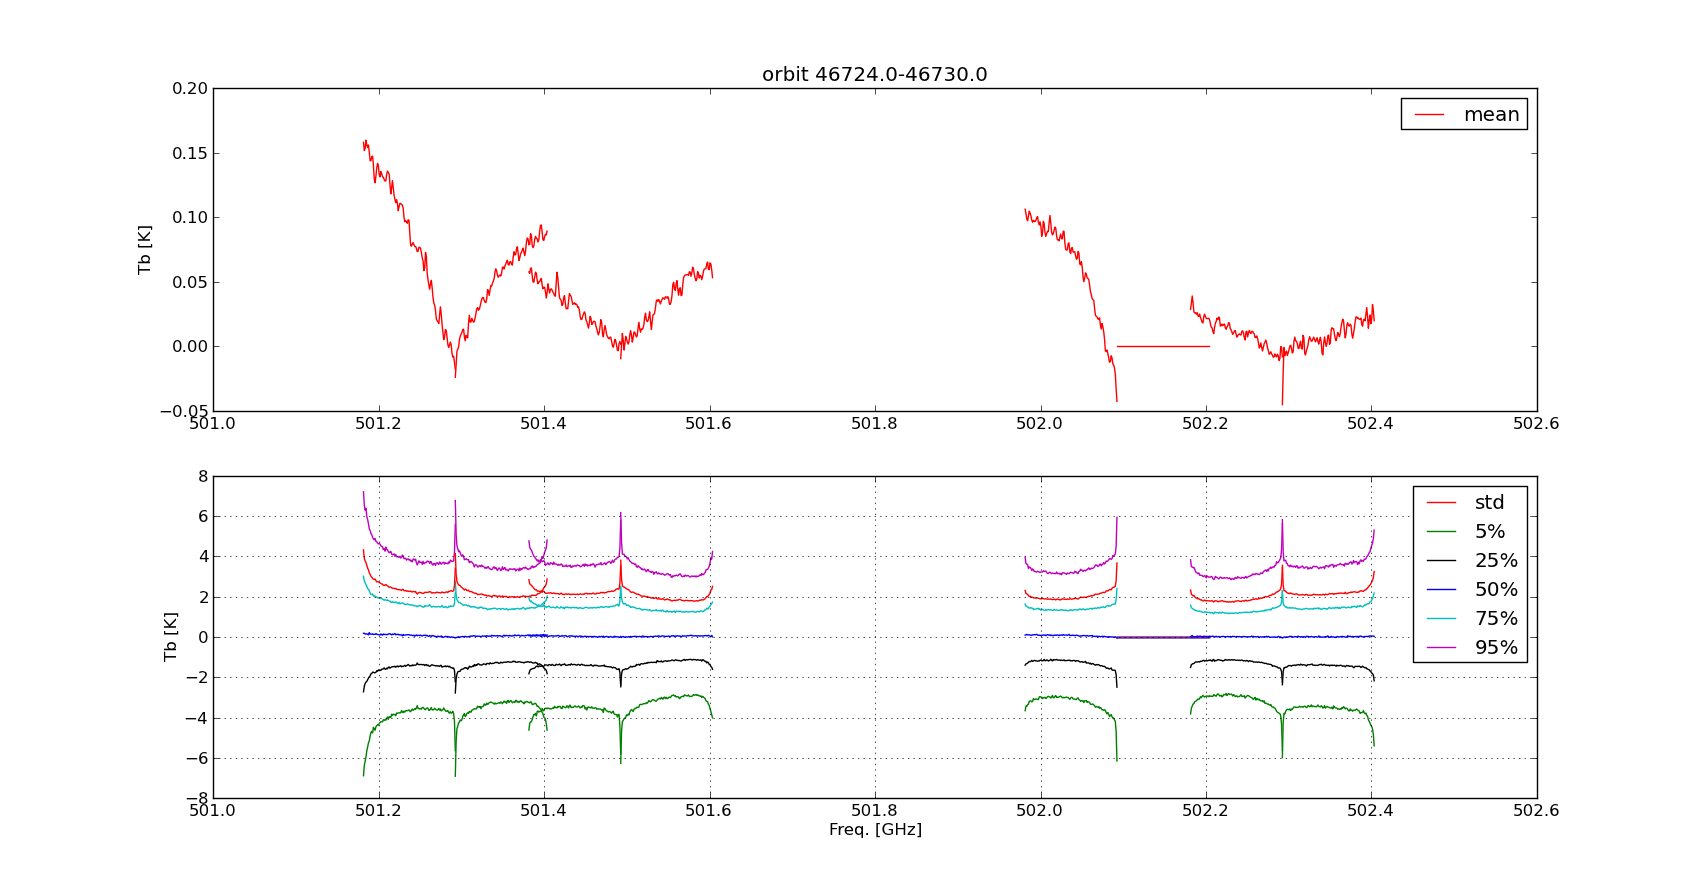
\includegraphics[scale=0.35]{study4linear.png}\\
\caption{The upper panel shows a mean spectrum of calibrated
sky signals from AC2 stratospheric mode 1,
using linear interpolation. 
The lower panel show a standard deviation spectrum
and percentiles spectra.}
\label{fig:study4linear.png}
\end{figure}

The upper panel of Figure 1 shows a mean spectrum
of calibrated sky signals from 6 orbits (~10000 sky signals). 
It can clearly be seen
that this spectrum deviates from 0 K (approximately the true brightness 
temperature of the sky signal).

The lower panel shows some additional statistics.
The standard deviation of the spectrum is around 2 K,
which agrees well with the expected theoretical noise level
(\(\Delta T =T_{sys}/\sqrt{B*\tau} \approx 3000 K / \sqrt{2MHz*0.8s}=2.37 K\)).
The percentiles (for example the 25 and 75) are fairly evenly
displaced from the 50\% percentile (median),
which means that the errors are at least close to Gaussian
distributed.  
The median has the same pattern as the mean (which is hard to see
due to the scale).

The reason for the median deviation from 0 K is most likely due to 
that the gain does not vary
completely linearly with time between three sky signals
measurements.

\subsubsection{Quadratic interpolation setup}
\begin{figure}[!t]
\centering
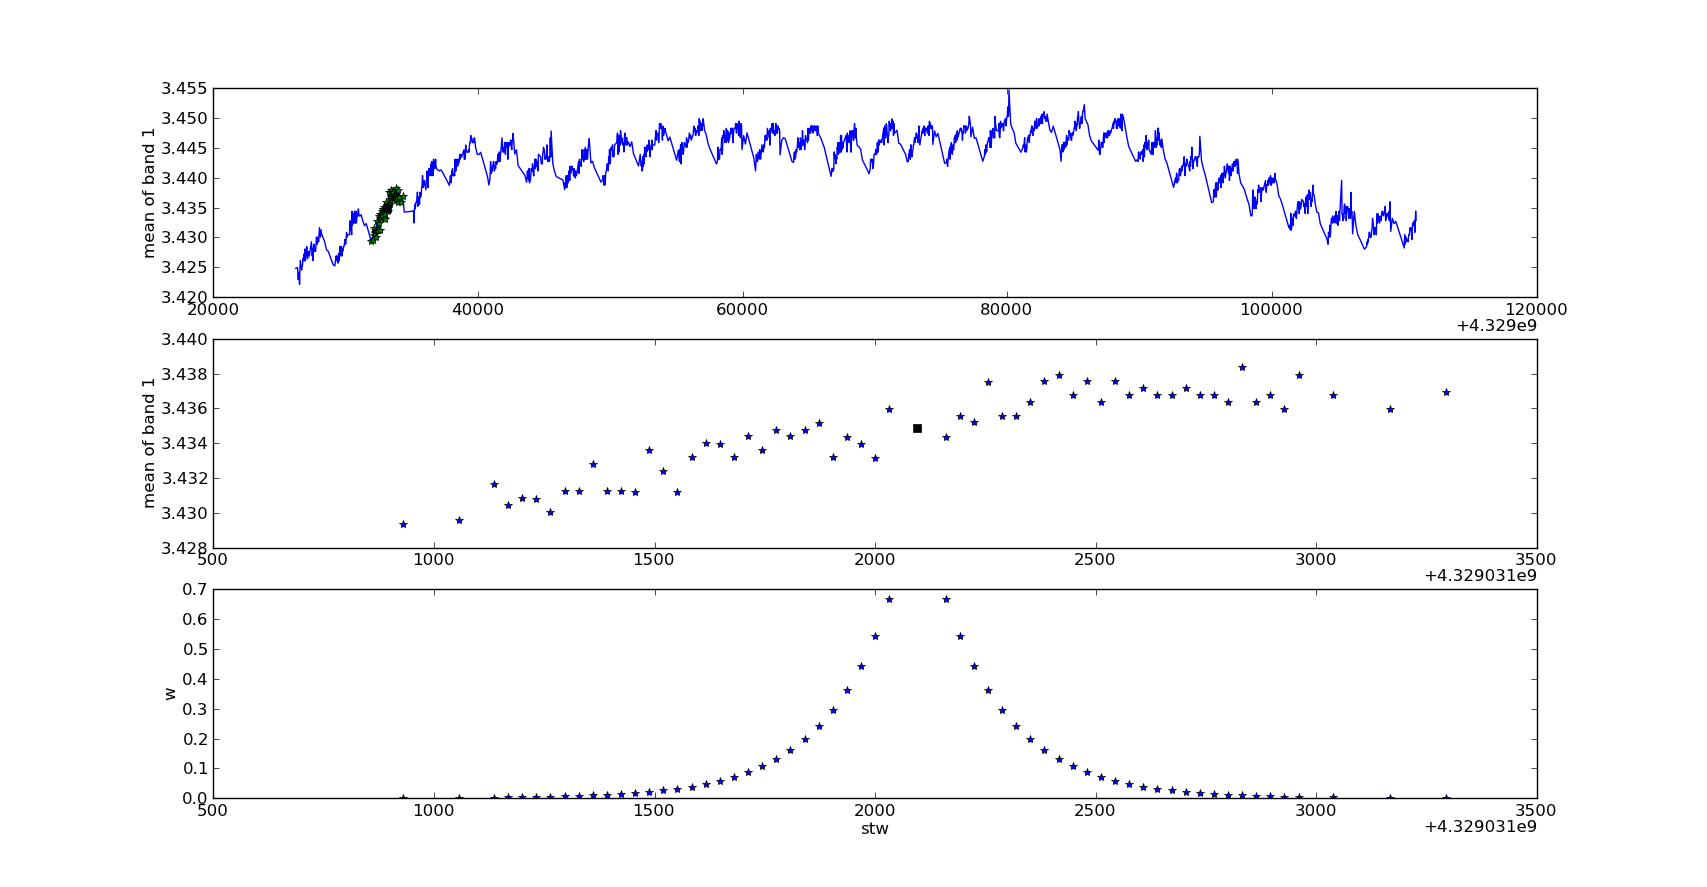
\includegraphics[scale=0.35]{study4_dem.png}\\
\caption{The upper panel shows mean of band1 of level1a data
from several scans.
The middle panel shows a zoom in of the black dots in the upper panel,
and the black square is the fitted value
(the fit is performed for each channel).
The lower panel shows the corresponding weights (x=8) of each measurement 
in the fit. }
\label{fig:study4_dem.png}
\end{figure}

The quadratic fit of a reference measurement at time \(t\)
is done in the following way (see Figure 2).  
We first find out the time-interval \(\Delta T\) of the scan that
the measurement belongs to. 
In the fit, we then consider all reference measurements
that where performed during the time interval 
\(t-\Delta T\) to \(t+\Delta T\). 
The weighting parameter \(\lambda\) is then given
the value  \(\Delta T /x\), where we tested the performance
of several values of x (4,8,16,32,64,and 128).

\clearpage
\newpage
\subsubsection{Quadratic interpolation}
\begin{figure}[!t]
\centering
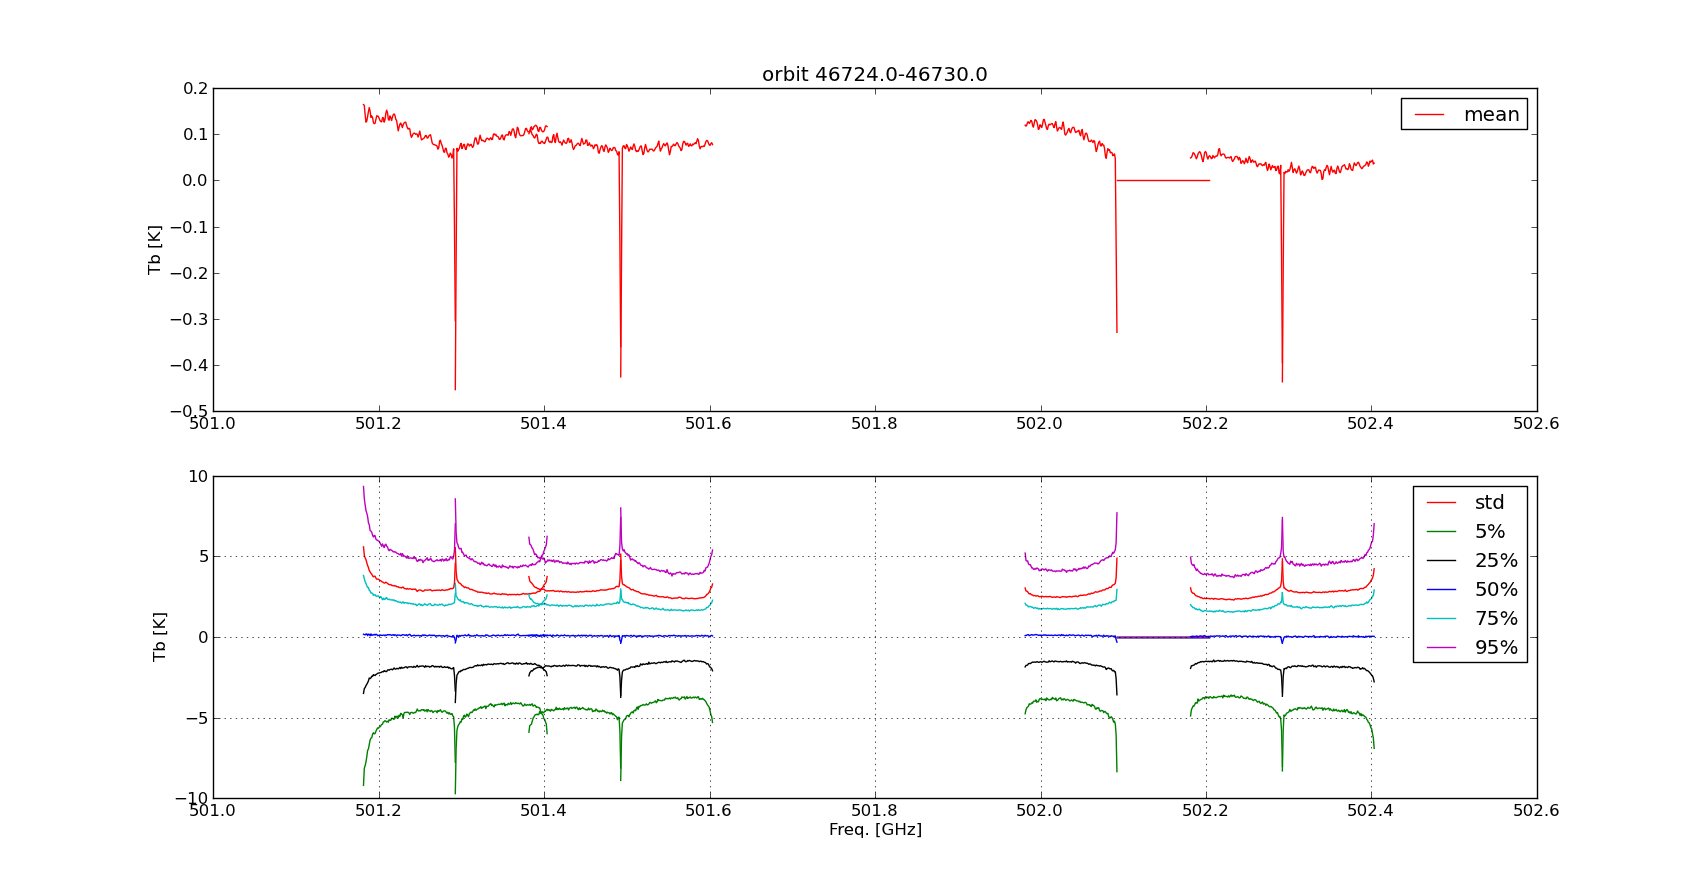
\includegraphics[scale=0.35]{study4_4.png}\\
\caption{The upper panel shows a mean spectrum of calibrated
sky signals from AC2 stratospheric mode 1,
using quadratic interpolation (x=4). 
The lower panel show a standard deviation spectrum
and percentiles spectra.}
\label{fig:study4_4.png}
\end{figure}

\begin{figure}[!t]
\centering
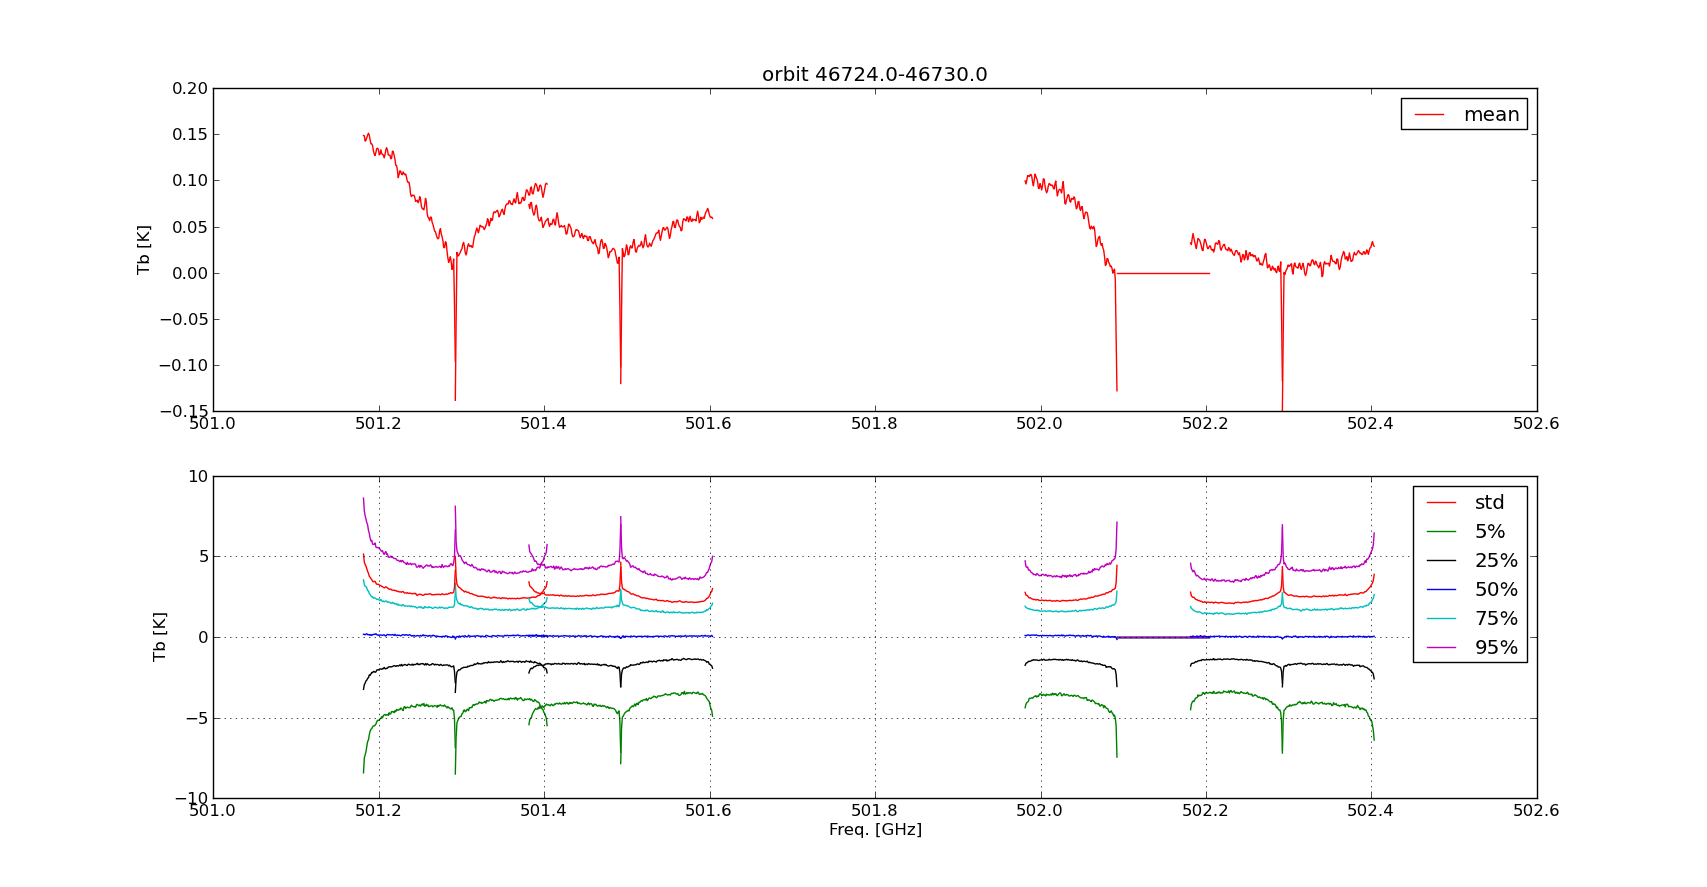
\includegraphics[scale=0.35]{study4_8.png}\\
\caption{The upper panel shows a mean spectrum of calibrated
sky signals from AC2 stratospheric mode 1,
using quadratic interpolation (x=8). 
The lower panel show a standard deviation spectrum
and percentiles spectra.}
\label{fig:study4_8.png}
\end{figure}

\begin{figure}[!t]
\centering
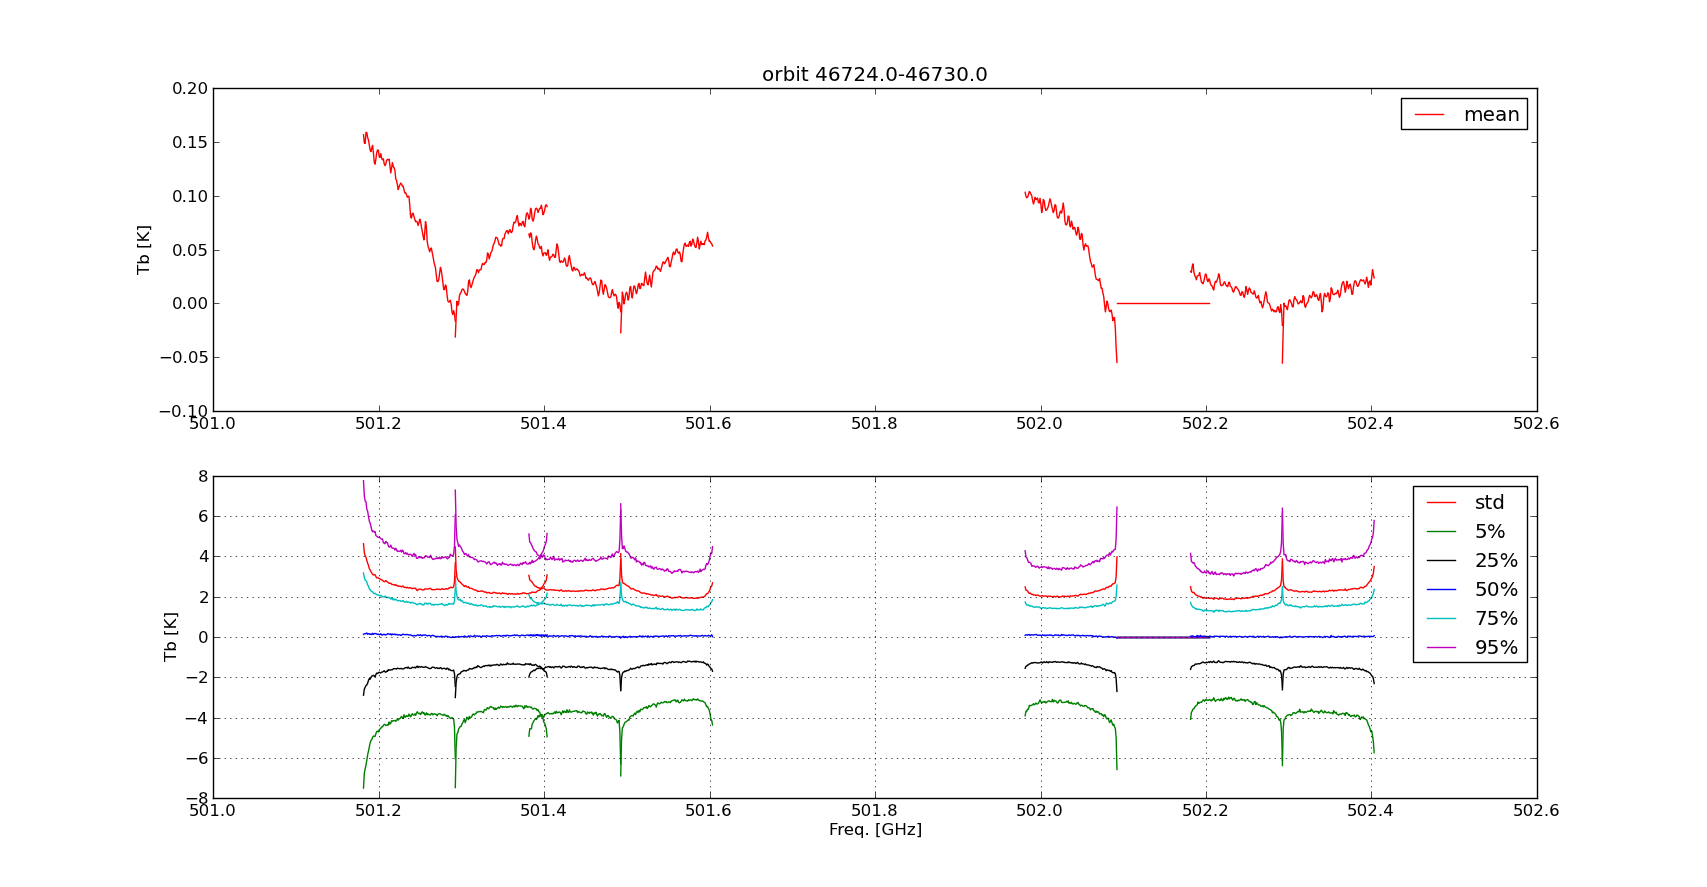
\includegraphics[scale=0.35]{study4_16.png}\\
\caption{The upper panel shows a mean spectrum of calibrated
sky signals from AC2 stratospheric mode 1,
using quadratic interpolation (x=16). 
The lower panel show a standard deviation spectrum
and percentiles spectra.}
\label{fig:study4_16.png}
\end{figure}

\begin{figure}[!t]
\centering
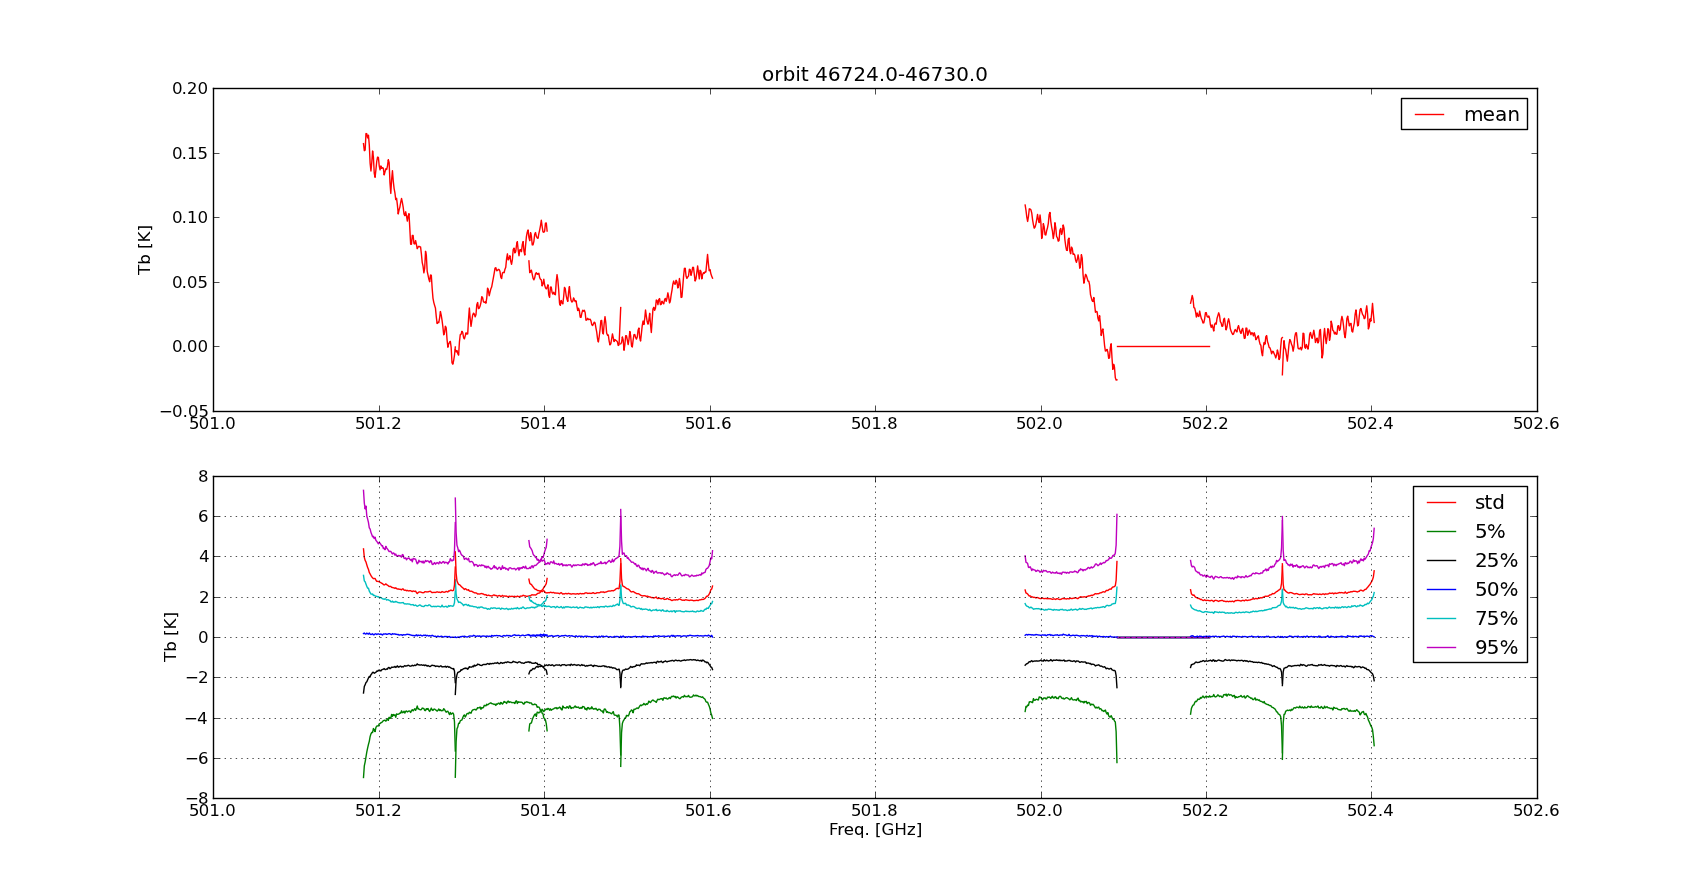
\includegraphics[scale=0.35]{study4_32.png}\\
\caption{The upper panel shows a mean spectrum of calibrated
sky signals from AC2 stratospheric mode 1,
using quadratic interpolation (x=32). 
The lower panel show a standard deviation spectrum
and percentiles spectra.}
\label{fig:study4_32.png}
\end{figure}

\begin{figure}[!t]
\centering
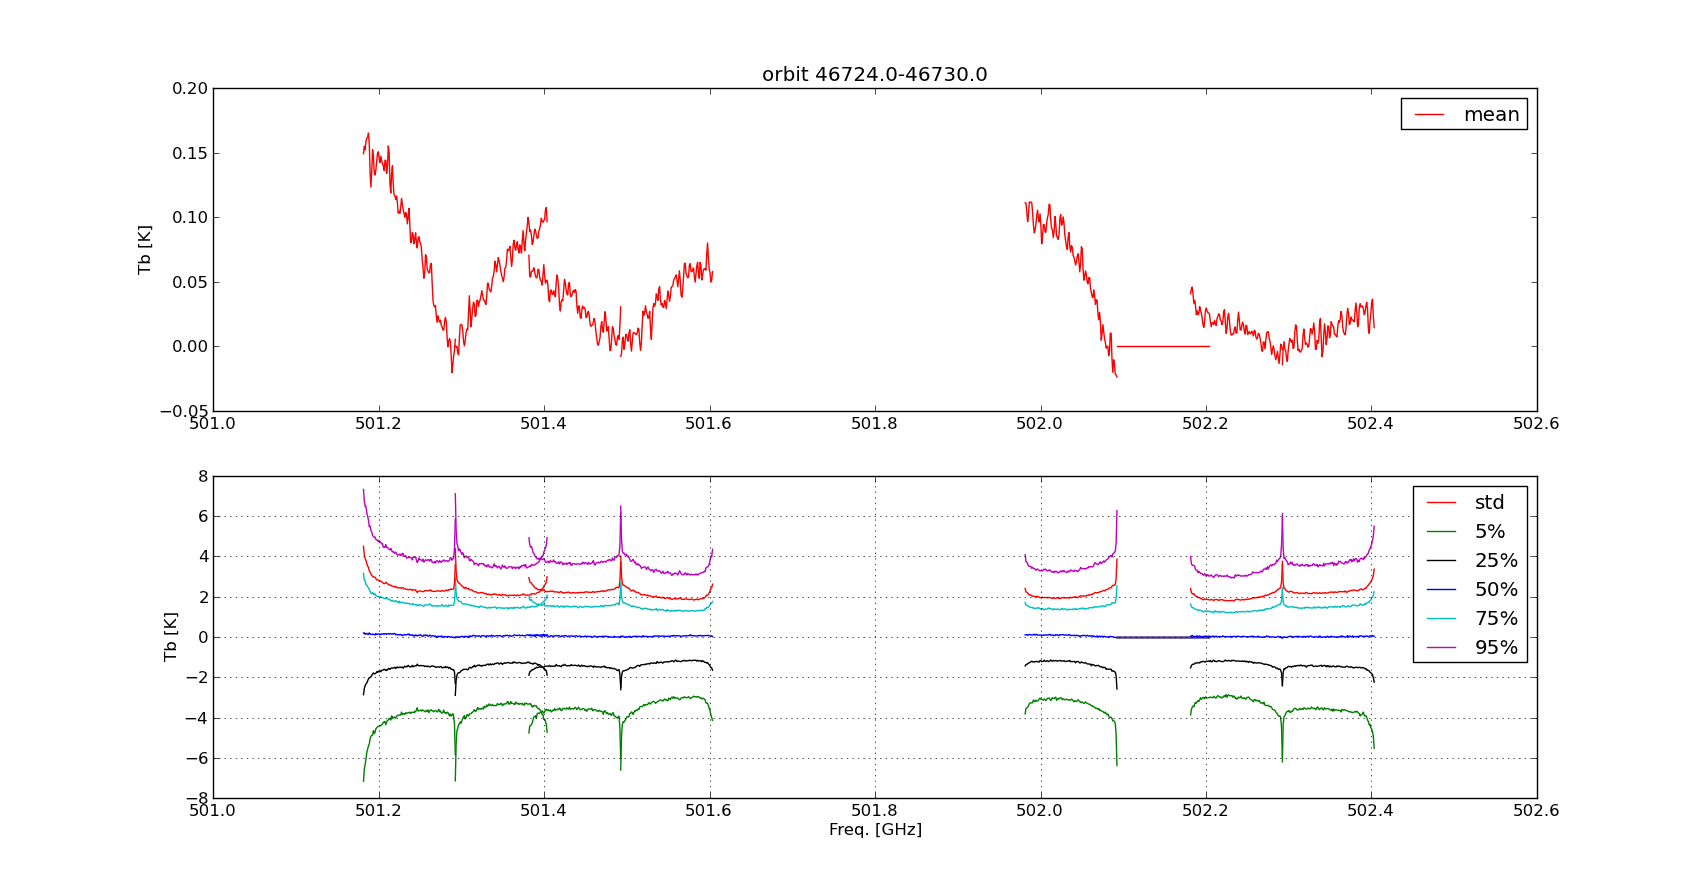
\includegraphics[scale=0.35]{study4_64.png}\\
\caption{The upper panel shows a mean spectrum of calibrated
sky signals from AC2 stratospheric mode 1,
using quadratic interpolation (x=64). 
The lower panel show a standard deviation spectrum
and percentiles spectra.}
\label{fig:study4_64.png}
\end{figure}

\begin{figure}[!t]
\centering
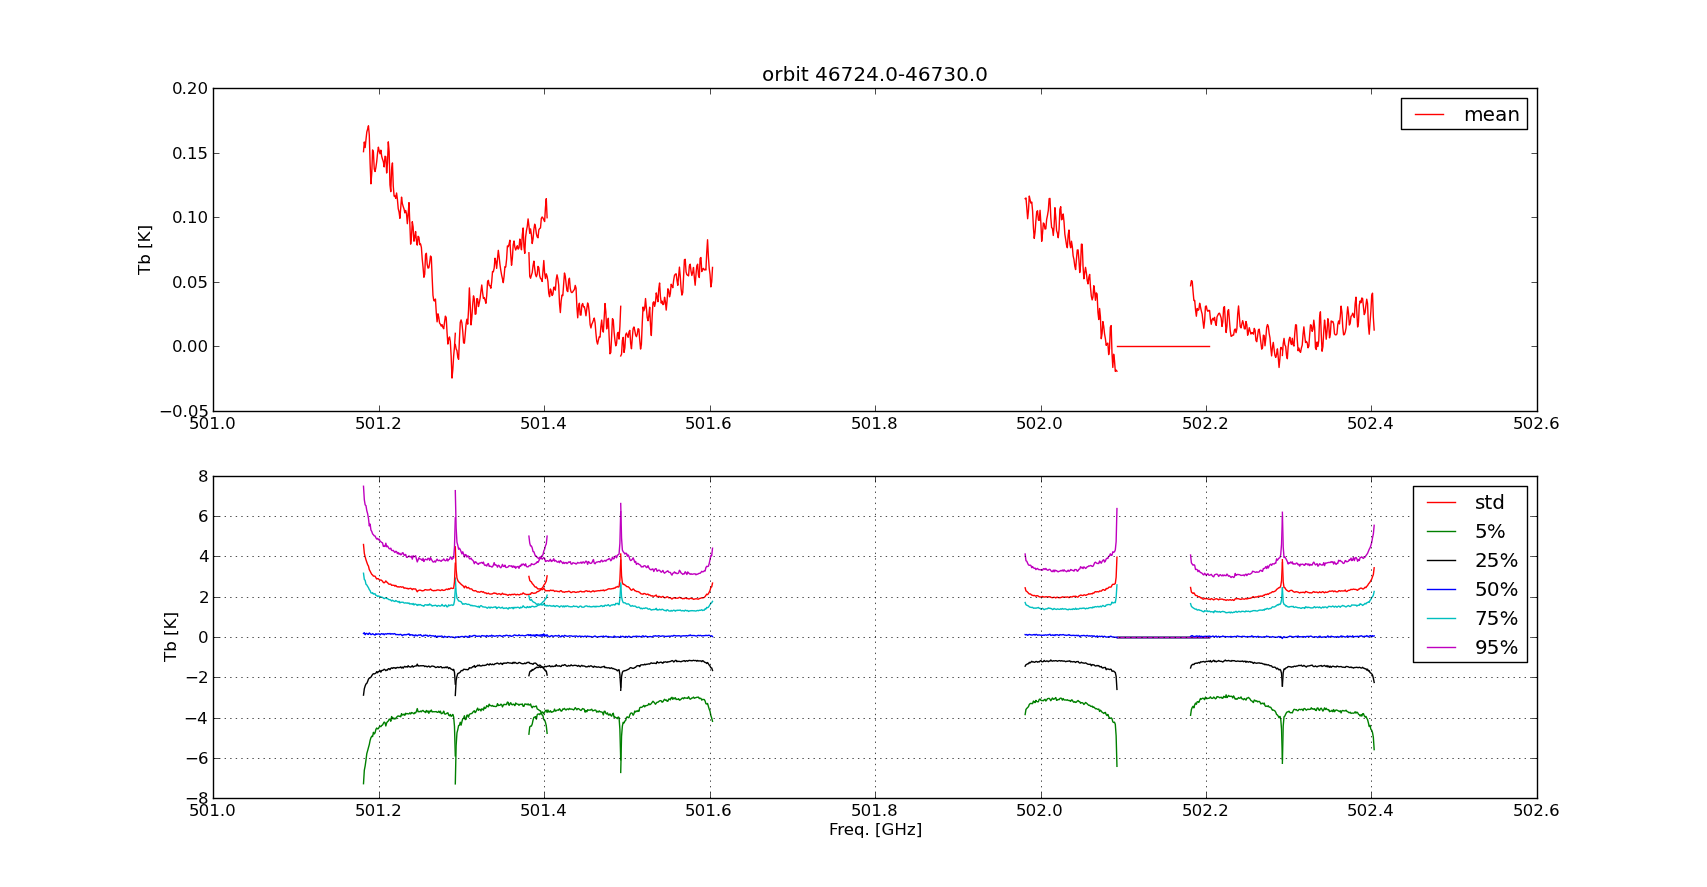
\includegraphics[scale=0.35]{study4_128.png}\\
\caption{The upper panel shows a mean spectrum of calibrated
sky signals from AC2 stratospheric mode 1,
using quadratic interpolation (x=128). 
The lower panel show a standard deviation spectrum
and percentiles spectra.}
\label{fig:study4_.png}
\end{figure}

Figures 3 to 8 show similar data as Figure 1 but using quadratic
interpolation with different setups
(weight parameter \(\lambda = \Delta T /x, x=4,8,16,32,64,128\)). 
In general, the results from the quadratic interpolations
are very similar as the result from the linear interpolation.
The same pattern in mean and median values are observed, and
similar distributions of data.
The result from x=32 setup seems to be slightly better
than for other values of x in terms of standard deviation,
and the results agree very well with the result from linear interpolation.
For such high value of \(x\) fairly few number of data
points are effectively used in the fit (see Figure 9).
Figure 9 indicates that the fit in this case should be 
very close to a linear interpolation.

   

\begin{figure}[!t]
\centering
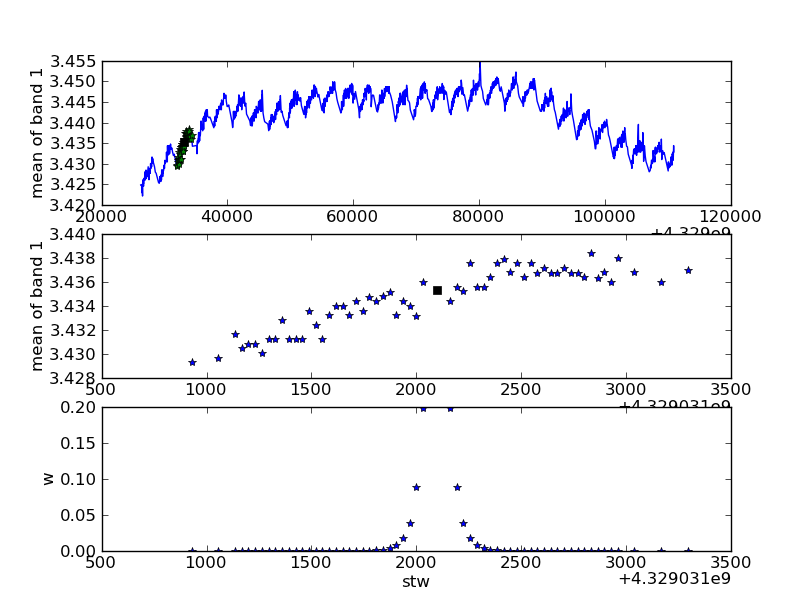
\includegraphics[scale=0.35]{study4_demo32.png}\\
\caption{The upper panel shows mean of band1 of level1a data
from several scans.
The middle panel shows a zoom in of the black dots in the upper panel,
and the black square is the fitted value
(the fit is performed for each channel). 
The lower panel shows the corresponding weights (x=32) of each measurement 
in the fit. }
\label{fig:study4_dem32.png}
\end{figure}

